% Sezione per il report di sintesi

\section{Sintesi}

La sintesi del componente descritto in VHDL attraverso Vivado ha generato i risultati riportati di seguito.

\subsection{Report di timing}
Il report di timing illustra come sia rispettato il constraint definito (ovvero che il sistema deve funzionare con un tempo di clock di al pi\`u 100ns). \`E riportato il riassunto del report:
\begin{verbatim}
--------------------------------------------------------------------
| Design Timing Summary
| ---------------------
--------------------------------------------------------------------

 WNS(ns)      TNS(ns)   TNS Failing Endpoints   TNS Total Endpoints       
 -------      -------   ---------------------   -------------------        
  96.767        0.000                       0                    77      

 WHS(ns)      THS(ns)   THS Failing Endpoints   THS Total Endpoints     
 -------      -------   ---------------------   -------------------     
   0.144        0.000                       0                    77  

WPWS(ns)     TPWS(ns)  TPWS Failing Endpoints  TPWS Total Endpoints
--------     --------  ----------------------  --------------------
   4.500        0.000                       0                    33

All user specified timing constraints are met.
\end{verbatim}

In particolare il WNS \`e calcolato come $max(required\_time - arrival\_time)$ per la propagazione dei segnali; questo implica che, relativamente a questo parametro, \`e possibile diminuire il tempo di clock fino a circa 4ns senza che il tempo sia insufficiente per la propagazione.

\newpage

\subsection{Report di utilizzo}

Nel report di utilizzo \`e stato possibile valutare il numero di componenti utilizzati; in particolare per i registri non sono stati riportati latch:
\begin{verbatim}
+-------------------------+------+-------+-----------+-------+
|        Site Type        | Used | Fixed | Available | Util% |
+-------------------------+------+-------+-----------+-------+
| Slice Registers         |   37 |     0 |    269200 |  0.01 |
|   Register as Flip Flop |   37 |     0 |    269200 |  0.01 |
|   Register as Latch     |    0 |     0 |    269200 |  0.00 |
+-------------------------+------+-------+-----------+-------+
\end{verbatim}

Nella lista di primitives si pu\`o invece notare che vengono utilizzati esclusivamente flip-flop di tipo D (FDCE e FDPE).
\begin{verbatim}
+----------+------+---------------------+
| Ref Name | Used | Functional Category |
+----------+------+---------------------+
| FDCE     |   35 |        Flop & Latch |
| OBUF     |   27 |                  IO |
| LUT2     |   12 |                 LUT |
| IBUF     |   11 |                  IO |
| LUT4     |    8 |                 LUT |
| LUT5     |    7 |                 LUT |
| LUT3     |    7 |                 LUT |
| LUT6     |    4 |                 LUT |
| FDPE     |    2 |        Flop & Latch |
| CARRY4   |    2 |          CarryLogic |
| BUFG     |    1 |               Clock |
+----------+------+---------------------+
\end{verbatim}

Le connessioni dei componenti sono mostrate in Figura \ref{schema}.

\begin{landscape}
	\begin{figure}
		\centering
		{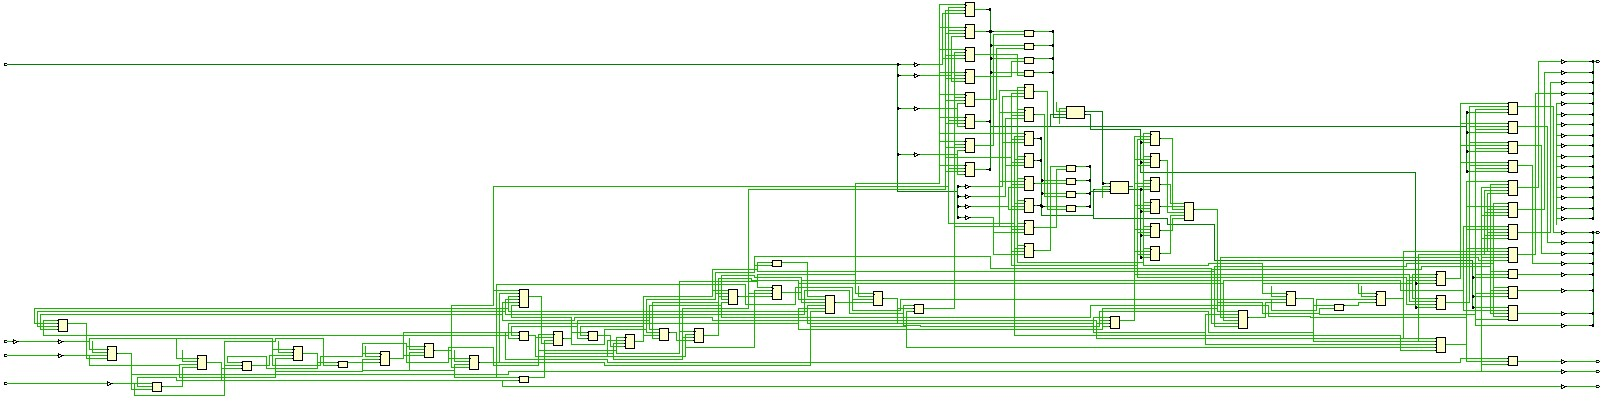
\includegraphics[scale=0.53,keepaspectratio]
			{schematic.jpg}}
		\caption{Schema sintetizzato}
		\label{schema}
	\end{figure}
\end{landscape}